\chapter{Description and Evaluation of Current Work}
\section{Introduction}
Partial work on exploring pre-processing techniques, useful features and classifiers has been done before data is collected from real subjects. The tools and approaches applied for the current stage and the associated results are shown and evaluated as below.

\section{System architecture}
The system architecture consists of three major parts as shown in Figure \ref{fig:system_architecture}. Data preparation and pre-processing are included in the first part. The pre-processed data is then passed to the second part of the system for feature extraction to obtain the essence of the signal. The last part of the system is responsible for two jobs, classification and estimation. The classifier discriminates the segmentation based on the feature extracted and then estimates the respiration related information such as respiratory phase and frequency. 

\begin{figure}[h]
    \centerline{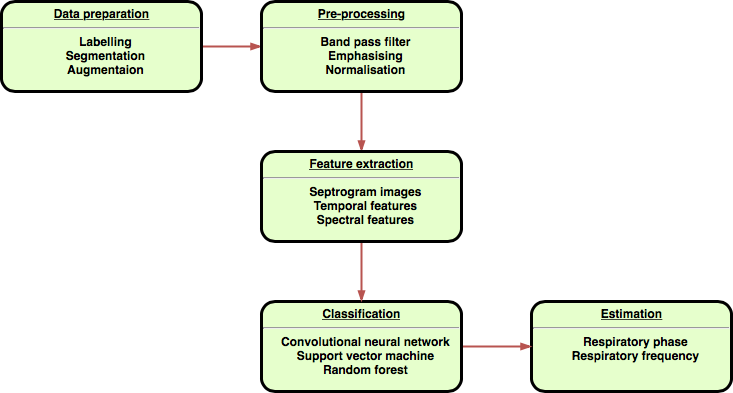
\includegraphics[scale=0.5]{figures/system_architecture.png}}
    \caption{system architecture}
    \label{fig:system_architecture}
\end{figure}


\section{Environment setup}
Instead of developing the system on the mobile platform straight away, the experiment was initially carried out on Colaboratory which is an cloud Jupyter Notebook environment and ideally for fast-prototyping. The experiment programs are written in Python which is commonly used in machine learning and deep learning community. Test data is stored on Google drive which is then mounted to the Jupyter notebook created on Colaboratory. This approach made the file management easy and reliable in the experimenting process. 

There were also various Python libraries used in this experiment. Librosa is a Python library focused on audio signal processing, it implements most of the popular signal processing approaches and enables easy access to the common spectral features. PyHHT and PyWT were also used for the implementation of Hilbert Huang transform and wavelet transform, respectively. Lastly, Matplotlib is great for visualisation and plots exporting. The spectrograms generated were used as an input for the convolution neural networks.

\section{Dataset preparation}
Prior to receiving the approval for the ethics application, the mock dataset was initially collected and created from the author during a short running outdoors. The test data consist of 4 .wav audio files which were recorded in 22150Hz with the Ios application named Audio Memos using IPhone 6 and the microphone in the original earpods . The duration of the files varies from 23 to 59 seconds. 

\subsection{Labelling}
The exhalation and inspiration segmentation contained in the audio file were manually labelled. However, the markers only represent when the exhalation and inhalation approximately begin. A more precised labelling could be obtained when having the referencing signal data from the actual data collection phase. An example of the test data with respiration phase labels is illustrated in Figure \ref{fig:audio_waveform}.

\begin{figure}[h]
    \centerline{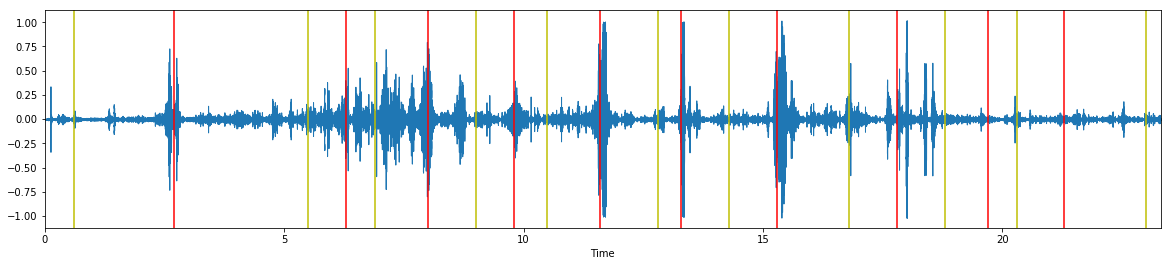
\includegraphics[scale=0.35]{figures/audio_waveform.png}}
    \caption{Audio signal with inhalation starting at yellow markers and exhalation starting at red markers }
    \label{fig:audio_waveform}
\end{figure}

\clearpage
\section{Pre-processing techniques}
The complete pre-processing pipieline consist of 4 steps which were inspired by these studies.\cite{Lei2014Content-basedFeatures}\cite{Niu2019AState}\cite{Ren2015Fine-grainedSmartphones} The completed results after applying the full pre-processing techniques is shown in Figure \ref{fig:fft_pipeline}.
\begin{figure}[h]
    \centerline{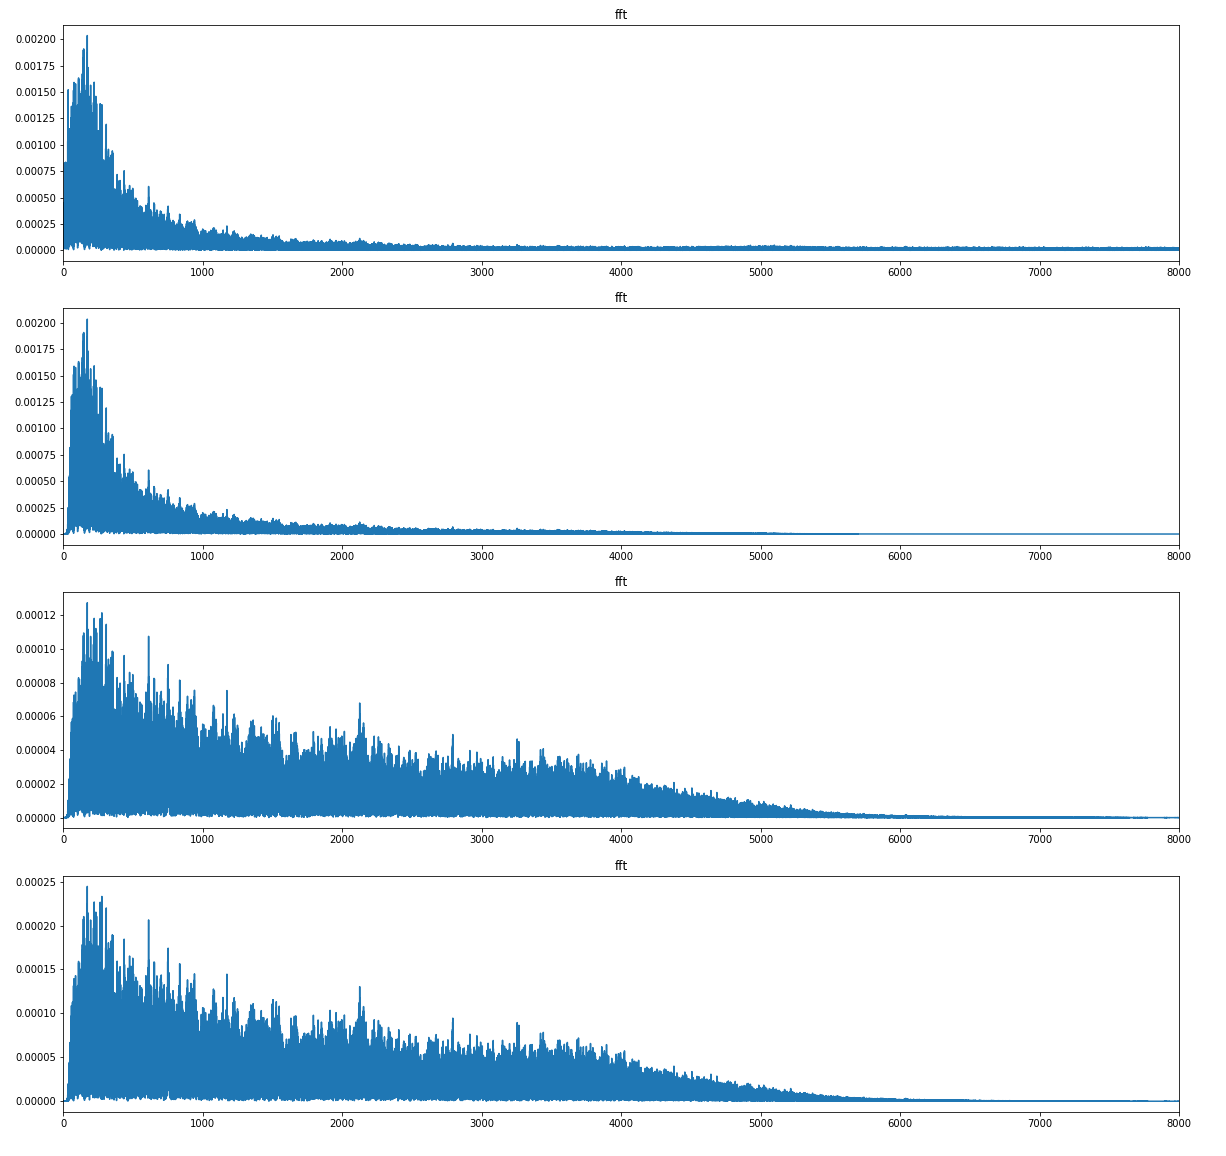
\includegraphics[scale=0.25]{figures/fft_pipeline.png}}
    \caption{The results of applying the full pre-processing techniques}
    \label{fig:fft_pipeline}
\end{figure}

\subsection{Band-pass filter}
The audio files was firstly passed into a band-pass filter which retained the signal with the frequency between 50Hz and 4000Hz. The frequencies that contained in these signals were also examined by applying fast Fourier transform as shown in . According to Figure \ref{fig:fft}, it was clearly shown that the major frequency range was 0-1000Hz.

\begin{figure}[h]
    \centerline{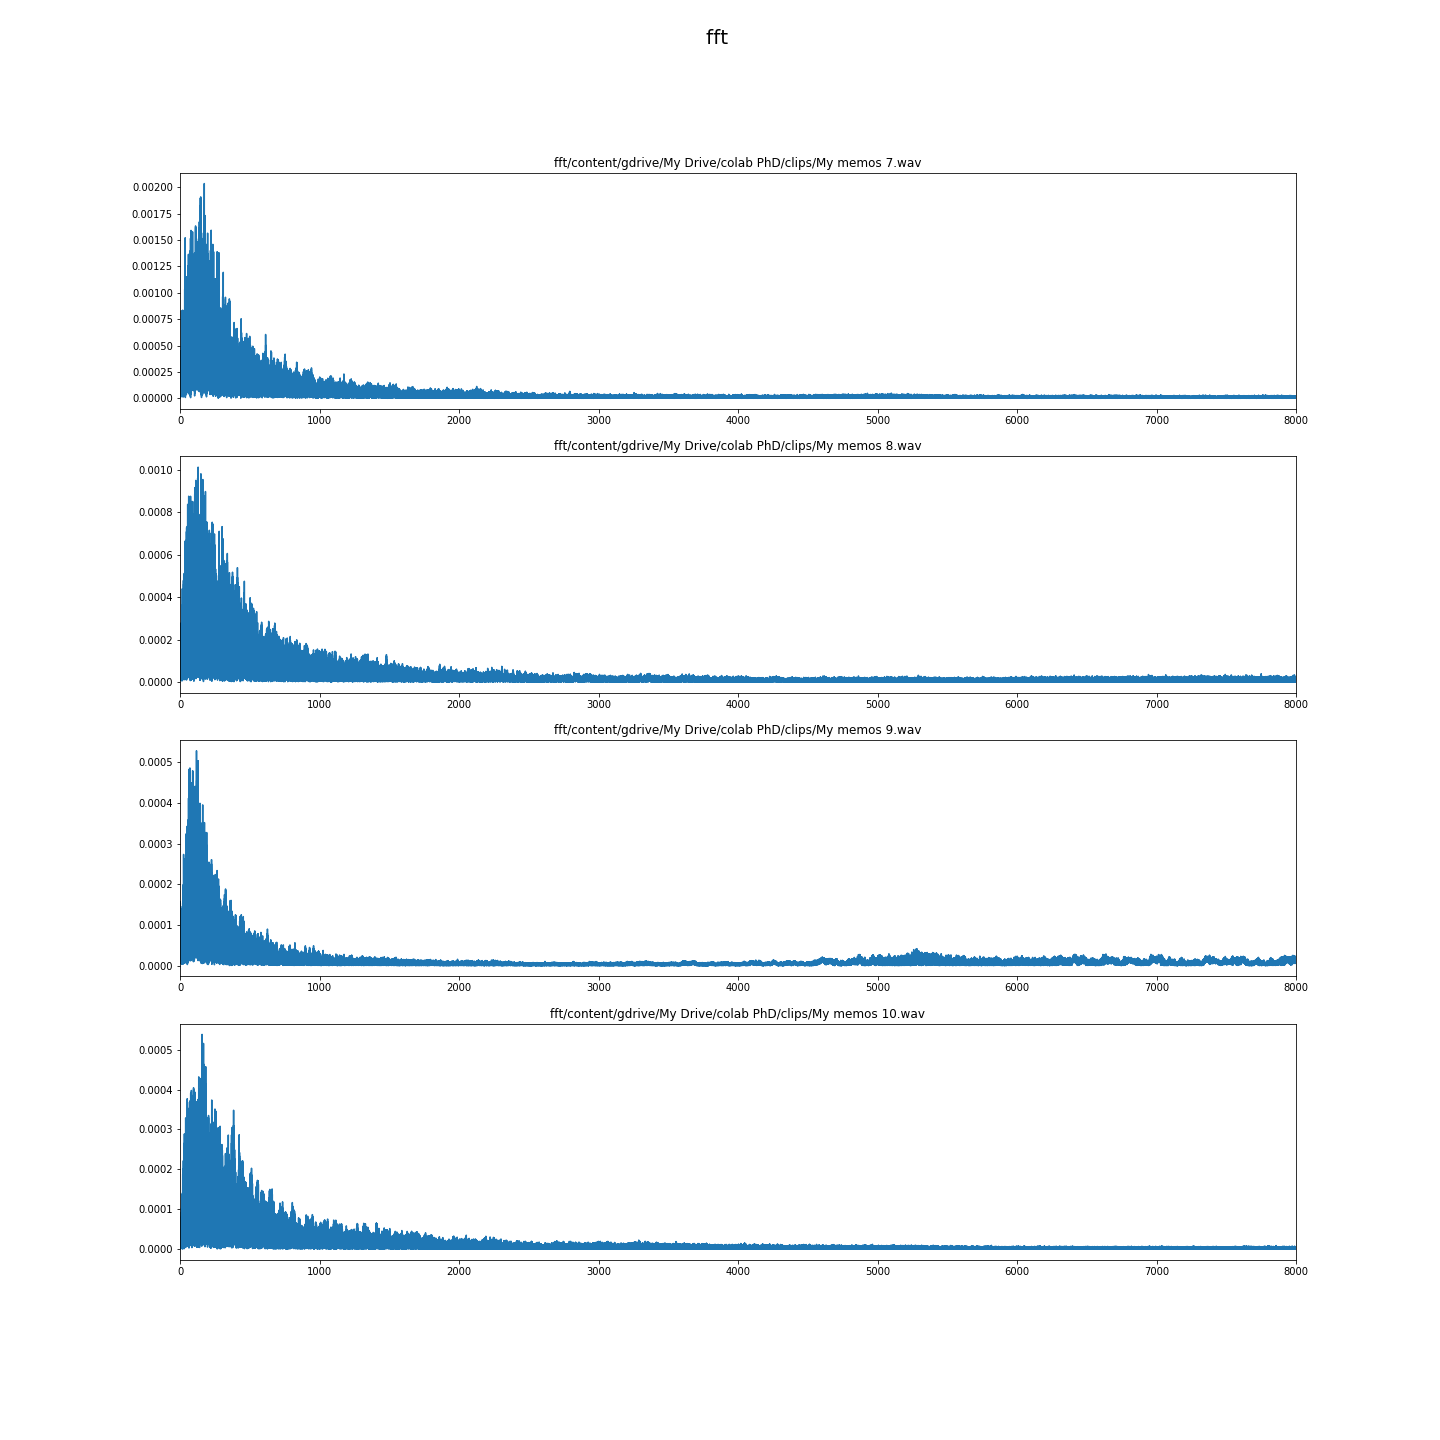
\includegraphics[scale=0.25]{figures/fft.png}}
    \caption{Frequency components of the 4 audio signals}
    \label{fig:fft}
\end{figure}
\subsection{Emphasising}
To overcome the radiation effects caused mostly by the lips, the signals were applied with a pre-emphasised filter to increase the amplitude of the components in high frequency range. The emphasising was completed by following the convertion below.

EQUATION HERE
\subsection{Normalisation}
Due to the variations of the devices used and the location the signals collected from, it is suggested to normalise the signal to have a stable performance.

\subsection{Segmentation}
For the purposes of feature extraction and classification, the signal data is segmented. Segmentations were created by including the following 1000 ms of data points after each of the markers. Each of the segmentation has 25\% of the data points overlapped with previous segmentation. For example, if an inhalation occurs in 13s, then the segmentation of this inhalation includes all of the data points from 13s to 14s. The segmentations created were very likely to include some of the non-respiration sound because of the subjective labelling. Therefore, it should affect the performance of the classifier described below.

\section{Feature extraction}
It aims to find the features which make the inhalation and exhalation most separable so the classifier could take advantage of them. 

\subsection{Spectral features}
As shown in last section, FFT shows the frequency range contained in a signal. However, it can demonstrate very little information regarding the relationship between time and frequency. There are some other frequency domain-based analysing approaches that fulfil this need by generating spectrograms. 

STFT is one of them. The idea behind short time Fourier transform is to apply fast Fourier transform on the signal with a sliding window of fixed length. The spetrogram is then converted to mel-sclaed spectrogram which has a better performance in modelling how humans percept low and high frequency. The comparison between STFT generated spectrogram and its mel-scaled spectrogram is shown in Figure \ref{fig:stft_mel-stft}. The mel-scaled spectrogram provides a more intuitive identification for exhalation than the original spectrogram. The red and yellow markers in the spectrogram represent when exhalation and inhalation begin. It clearly shows that most of the red markers perfectly align with one of the peak in the spectrogram. The red markers which do not associate with any peaks were also hard to distinguish through listening to the audio subjectivly. On the other hand, it is relatively impossible to recognise the inhalation through simply looking at the mel-scaled spectrogram.

\begin{figure}[h]
    \centerline{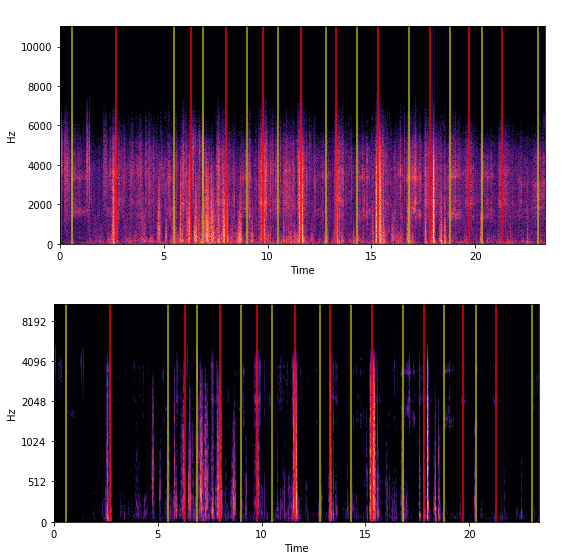
\includegraphics[scale=0.6]{figures/stft_mel-stft.png}}
    \caption{stft vs mel-stft}
    \label{fig:stft_mel-stft}
\end{figure}

However, STFT is not good for non-stationary signals. Also it has to balance the trade off between the time resolution and frequency resolution. Continuous wavelet transform is a solution to model the relationship between time and frequency of a non-stationary signal. Continuous wavelets transform is a great solution for transient signals since it has good resolution in time and poor resolution in frequency at high frequency. It would be helpful to capture the transients features by adopting continuous wavelet transform. Different wavelet functions influence the results of spectrogram generation. There were three kinds (Gaus, Mexh and Morl) of continuous wavelet function experimented and the results are shown in Figure \ref{fig:wavelet_functions}. It is fairly difficult to identify which wavelet function gives a better result in presenting the signal.
\begin{figure}[h]
    \centerline{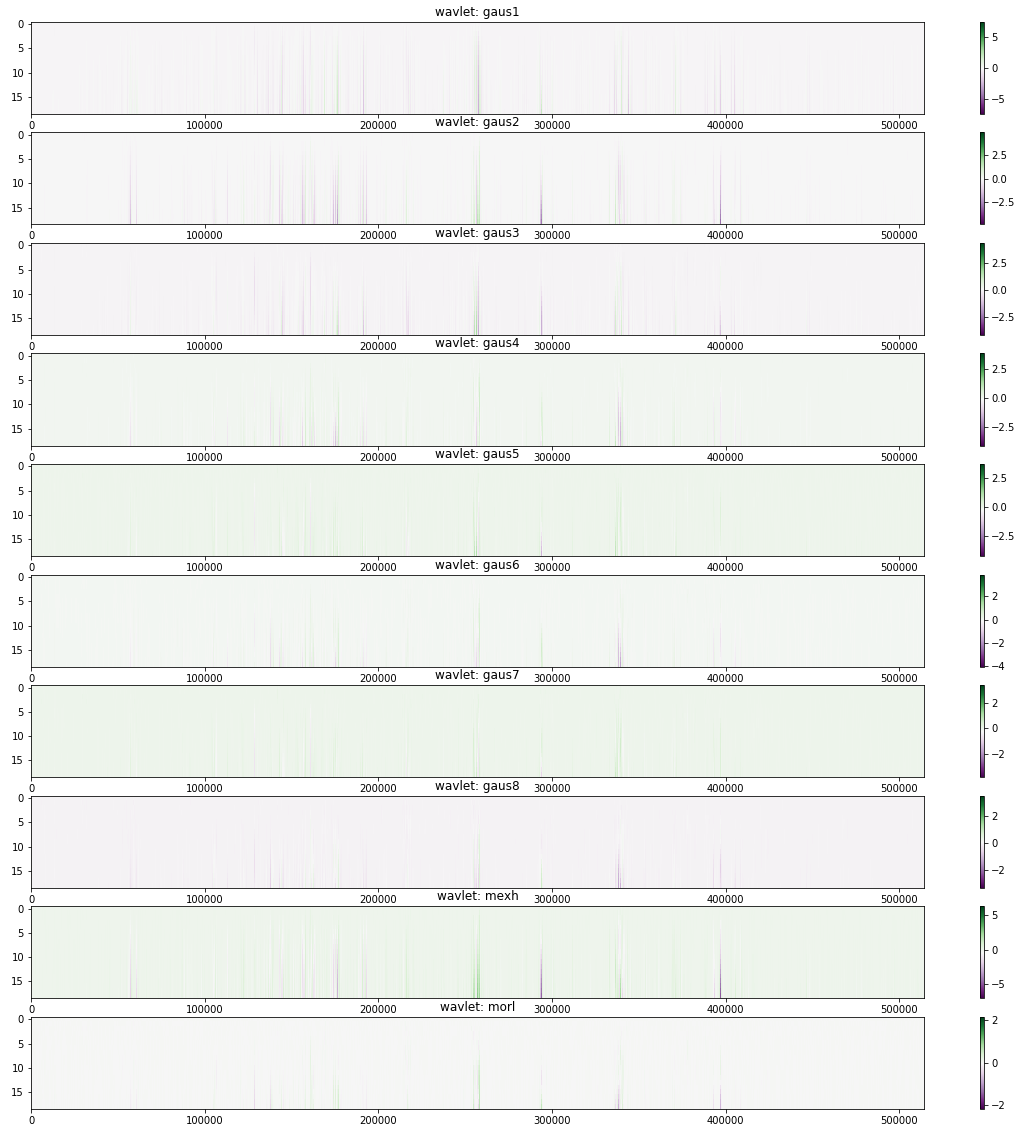
\includegraphics[scale=0.25]{figures/wavelet_trans_wav_func.png}}
    \caption{Applying different wavelet functions}
    \label{fig:wavelet_functions}
\end{figure}

\subsection{Temporal features}
Energy used for voiced-unvoiced segmentation discrimination to reduce computation cost

Training 

Testing
\subsection{Spectrogram generation}
In order to generate training data for CNN, the spectrogram of the audio files which represent the segmentations of inhalation and exhalation will be generated and saved in coresponding folders on Google drive for easy access from Colaboratory. In total, there were 51 inhalation segmentations and 54 exhalation segmentation which were created from four respiration sound files. 20\% of the segmentation were randomly selected and then used as valid data.

\subsubsection{Data augmentation}
The purpose of data augmentation is to increase the variety of the dataset especially when the dataset is small. Unlikely 

\section{Classification}
To quickly investigate the feasibility of classifying respiration sound using audio files generated spectrograms, thrid-party deep learning library FastAI was selected for implementation. Instead of training a nerual network from scratch, resnet18 which is a variation of convolutional neural network was used for the purpose of transfer learning. 

\begin{figure}[h]
    \centering
    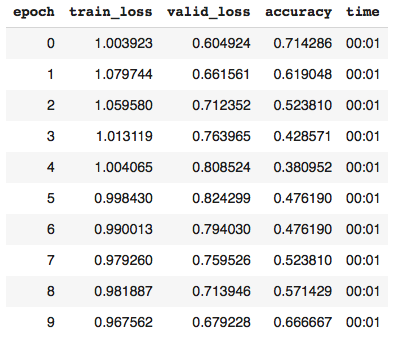
\includegraphics[scale=0.6]{figures/classification_results.png}
    \caption{Classification results}
    \label{fig:classification_results}
\end{figure}

Why the rate is low

pre-processing approach filtered out some wanted frequency components

dataset too small

structure

\section{Estimation}


